\documentclass[russian,utf8,emptystyle]{eskdtext}

\newcommand{\No}{\textnumero} % костыль для фикса ошибки

\ESKDdepartment{Федеральное государственное бюджетное образовательное учреждение высшего профессионального образования}
\ESKDcompany{Московский государственный технический университет им. Н. Э. Баумана}
\ESKDclassCode{23 0102}
\ESKDtitle{Лабораторная работа 1-3}
\ESKDdocName{по курсу <<Системы передачи данных>>}
\ESKDauthor{Гуща~А.~В.}
\ESKDtitleApprovedBy{~}{Антонов А.И.}
\ESKDtitleAgreedBy{~}{Антонов А.И.}
\ESKDtitleDesignedBy{Студент группы ИУ5-92}{Гуща~А.~В}

\usepackage{multirow}
\usepackage{tabularx}
\usepackage{tabularx,ragged2e}
\usepackage{pdfpages}
\renewcommand\tabularxcolumn[1]{>{\Centering}p{#1}}
\newcommand\abs[1]{\left|#1\right|}

\usepackage{longtable,tabu}

\usepackage{geometry}
\geometry{footskip = 1cm}

\pagenumbering{arabic}
\pagestyle{plain}

\usepackage{setspace}
\usepackage{enumitem}

\usepackage{xcolor}
\usepackage{listings}
\lstset{
    breaklines=true,
    postbreak=\raisebox{0ex}[0ex][0ex]{\ensuremath{\color{red}\hookrightarrow\space}},
    extendedchars=\true,
    basicstyle=\small,
    inputencoding=utf8
}
\lstdefinelanguage{D}{
    keywords = {
    abstract,
    alias,
    align,
    asm,
    assert,
    auto,
    body,
    bool,
    break,
    byte,
    case,
    cast,
    catch,
    cdouble,
    cent,
    cfloat,
    char,
    class,
    const,
    continue,
    creal,
    dchar,
    debug,
    default,
    delegate,
    delete,
    deprecated,
    do,
    double,
    else,
    enum,
    export,
    extern,
    false,
    final,
    finally,
    float,
    for,
    foreach,
    foreach_reverse,
    function,
    goto,
    idouble,
    if,
    ifloat,
    immutable,
    import,
    in,
    inout,
    int,
    interface,
    invariant,
    ireal,
    is,
    lazy,
    long,
    macro,
    mixin,
    module,
    new,
    nothrow,
    null,
    out,
    override,
    package,
    pragma,
    private,
    protected,
    public,
    pure,
    real,
    ref,
    return,
    scope,
    shared,
    short,
    static,
    struct,
    super,
    switch,
    synchronized,
    template,
    this,
    throw,
    true, 
    try,
    typedef,
    typeid,
    typeof,
    ubyte,
    ucent,
    uint,
    ulong,
    union,
    unittest,
    ushort,
    version,
    void,
    volatile,
    wchar,
    while,
    with,
    __FILE__,
    __MODULE__,
    __LINE__,
    __FUNCTION__,
    __PRETTY_FUNCTION__,
    __gshared,
    __traits,
    __vector,
    __parameters,
    }
}

\begin{document}
\maketitle
%\includepdf[pages={1}]{title.pdf}

\tableofcontents
\clearpage

\section{Задание}

\begin{longtable}{p{2cm}|p{5cm}|p{1cm}|p{2cm}|p{2cm}|p{1.5cm}}
Вариант & Удаленный хост & Ping & Traceroute & Проверка сервисов & Запрос \\
\hline
7       & а-айсберг.рф   & +    &            & +                 & whois, lookup      \\
\end{longtable}

\section{Выполнение}
Выполним команду ping на хост а-айсберг.рф:
\begin{figure}[h!]
\centering
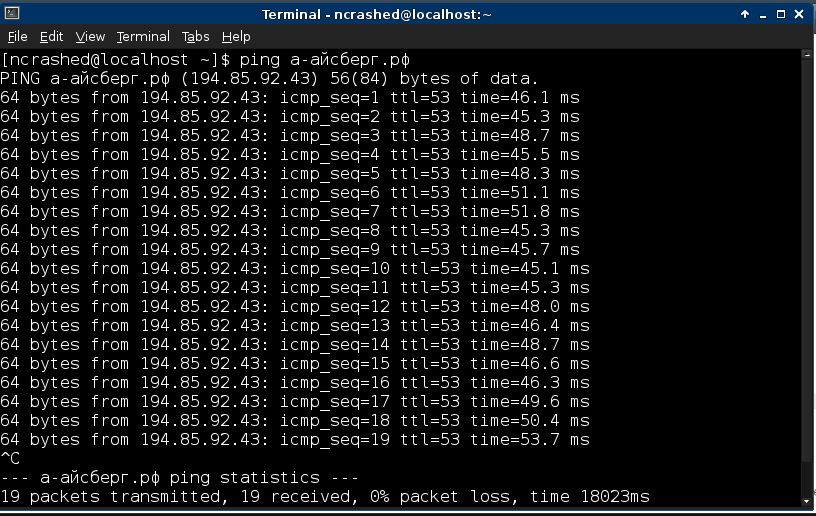
\includegraphics[width=0.7\textwidth]{001}
\end{figure}

Отловим все ICMP сообщения по адресу 194.85.92.43 через wireshark:
\begin{figure}[h!]
\centering
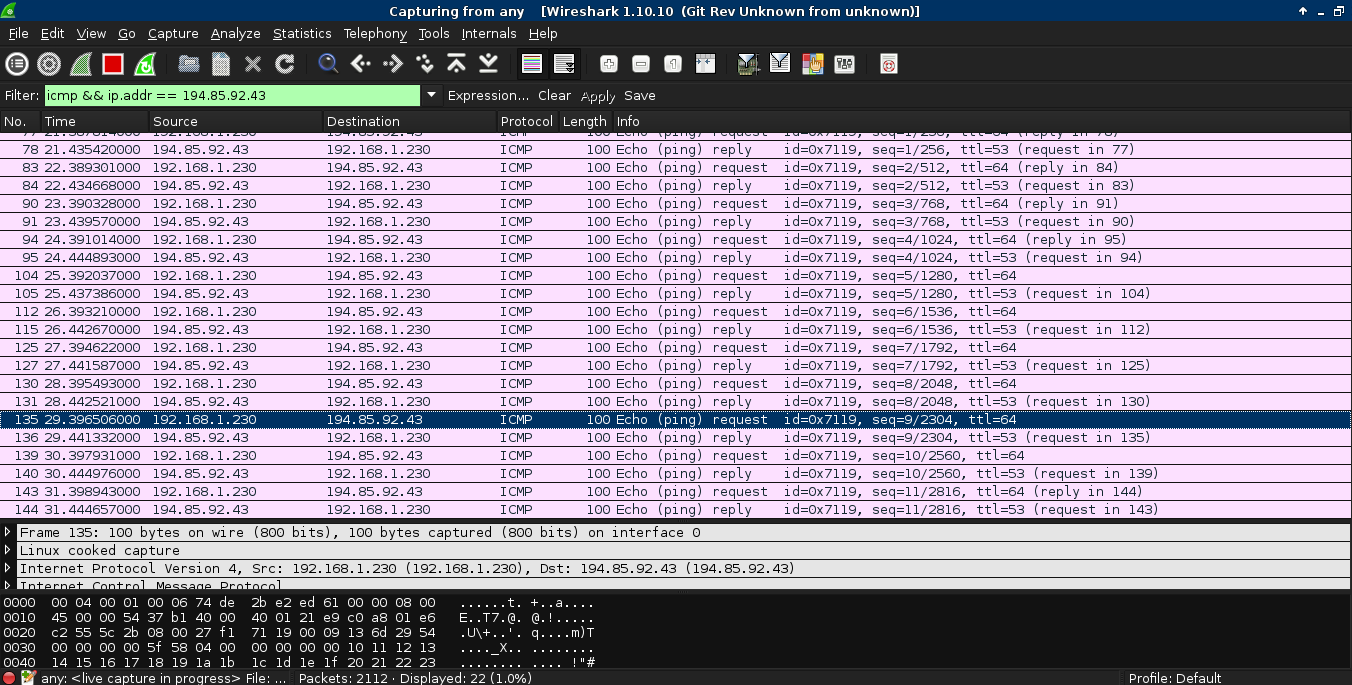
\includegraphics[width=1.0\textwidth]{002}
\end{figure}

Проведем подробный анализ содержимого пакета:
\begin{figure}[h!]
\centering
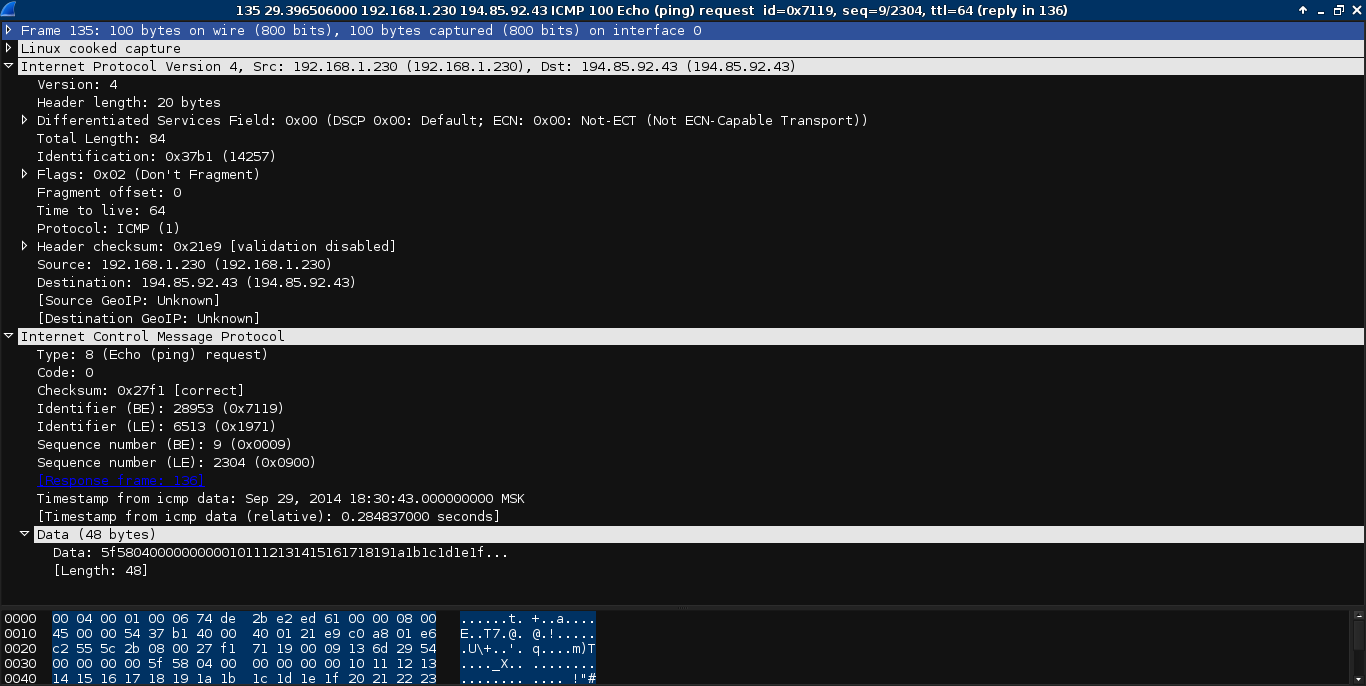
\includegraphics[width=1.0\textwidth]{003}
\end{figure}
\clearpage

Исходя из данной информации можно сделать выводы:
\begin{itemize}
\item Использовался ICMP поверх IPv4. В сообщении есть все поля из IP (адрес назначения и источника, время жизни, контрольная сумма и т.д.)
\item Тип ICMP сообщения 8, который означает эхо-запрос. Просмотр аналогичного сообщения ответа показывает Type равным 0, что означает ответ на полученное сообщение.
\end{itemize}

Используем команду traceroute:
\begin{figure}[h!]
\centering
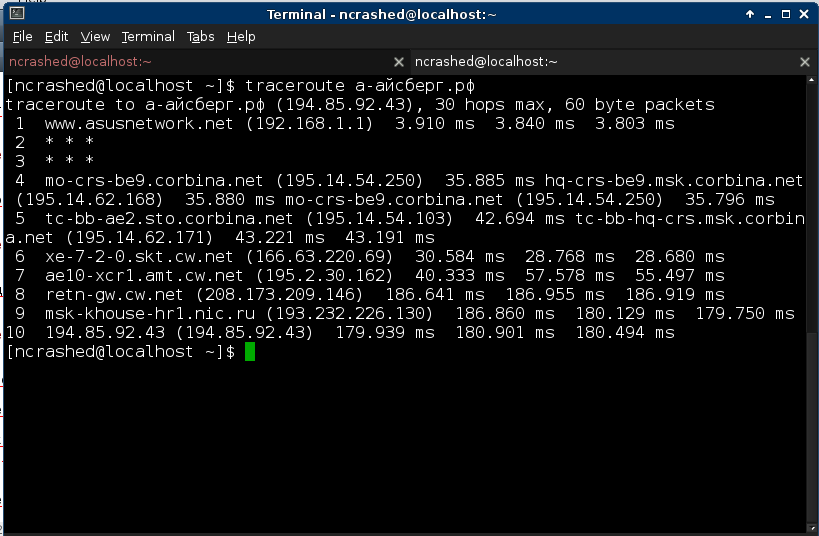
\includegraphics[width=0.7\textwidth]{004}
\end{figure}
\begin{figure}[h!]
\centering
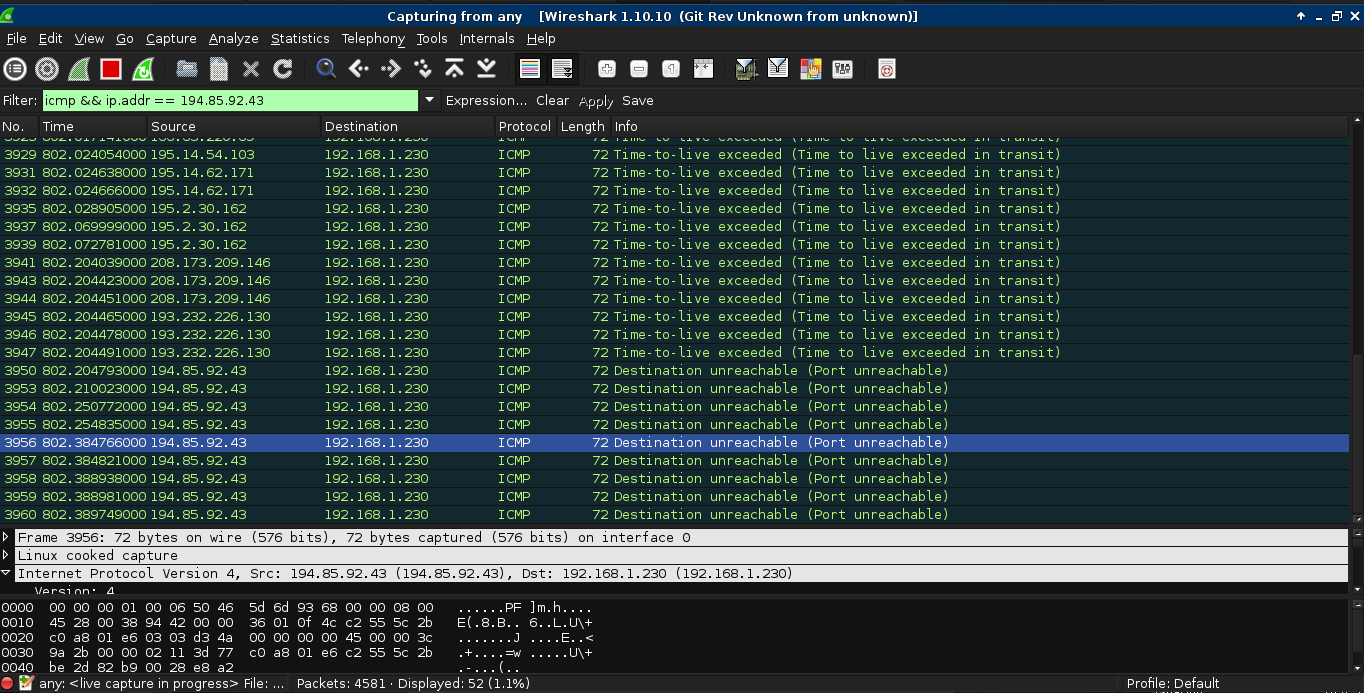
\includegraphics[width=\textwidth]{005}
\end{figure}

Traceroute отправляет пакеты с заранее малым значением TTL, которое постепенно увеличивается, что позволяет получать статистику о  узлах, через которые проходят пакеты. При уменьшении значения поля TTL до 0, отправителю отправляется сообщение-ошибка.

Это подтверждается на packet-flow графике:
\begin{figure}[h!]
\centering
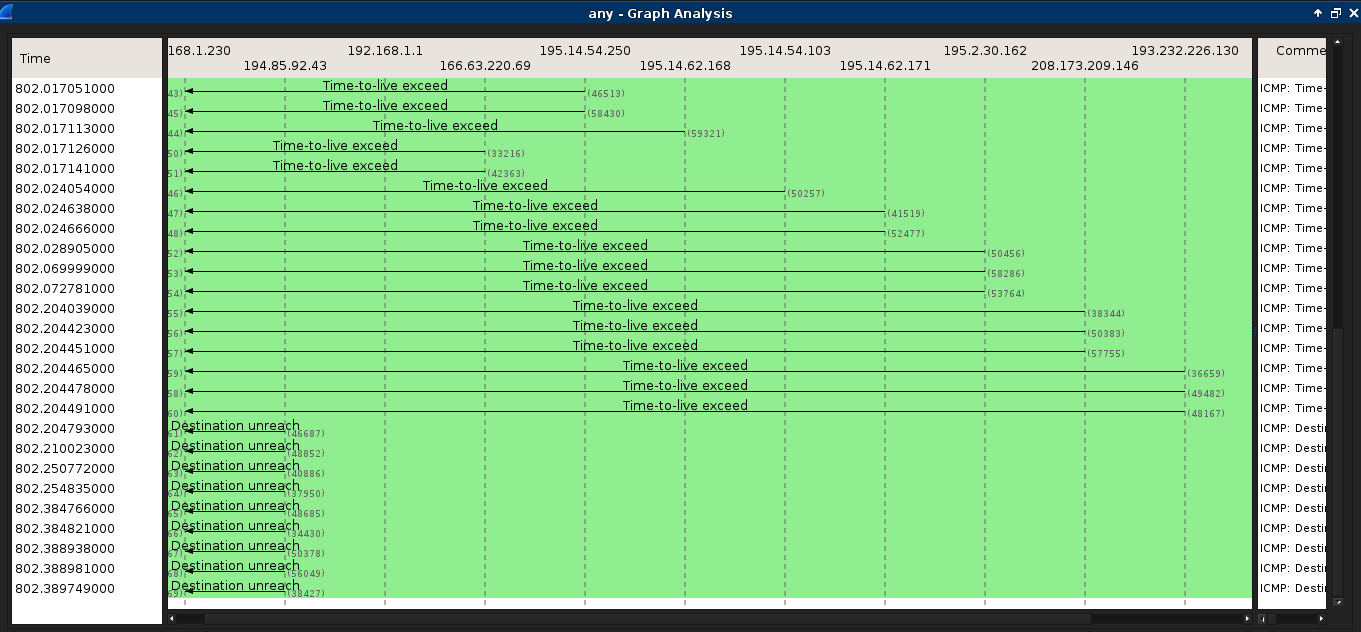
\includegraphics[width=\textwidth]{006}
\end{figure}

Проверим все сервисы и порты на хосте а-айсберг.рф с помощью утилиты nmap:
\begin{figure}[h!]
\centering
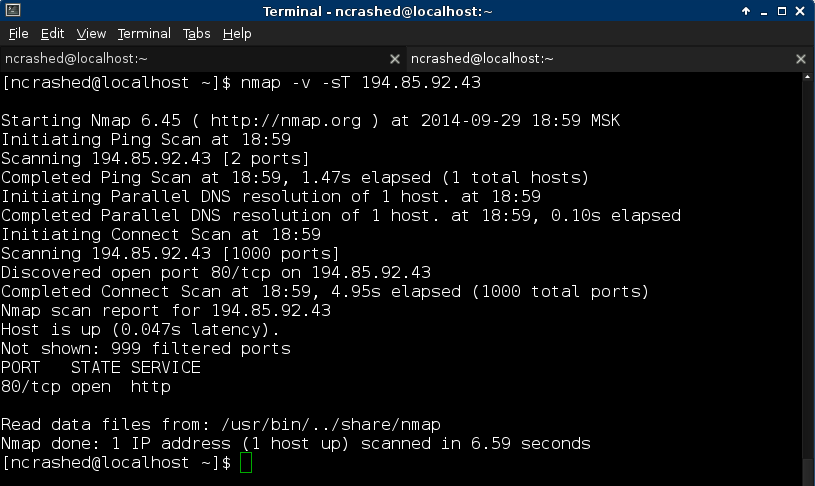
\includegraphics[width=0.7\textwidth]{007}
\end{figure}
Открыт только порт с номером 80 - HTTP порт.

Проверим доступные службы:
\begin{figure}[h!]
\centering
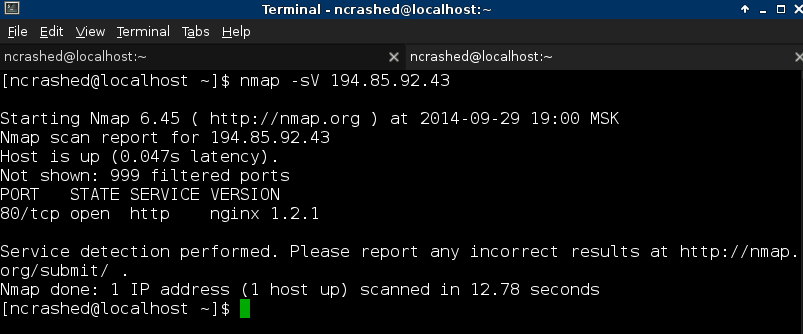
\includegraphics[width=0.7\textwidth]{008}
\end{figure}

После сканирования было выявлено, что на 80-м порту запущен веб сервер nginx.

Сделаем запрос whois:
\begin{figure}[h!]
\centering
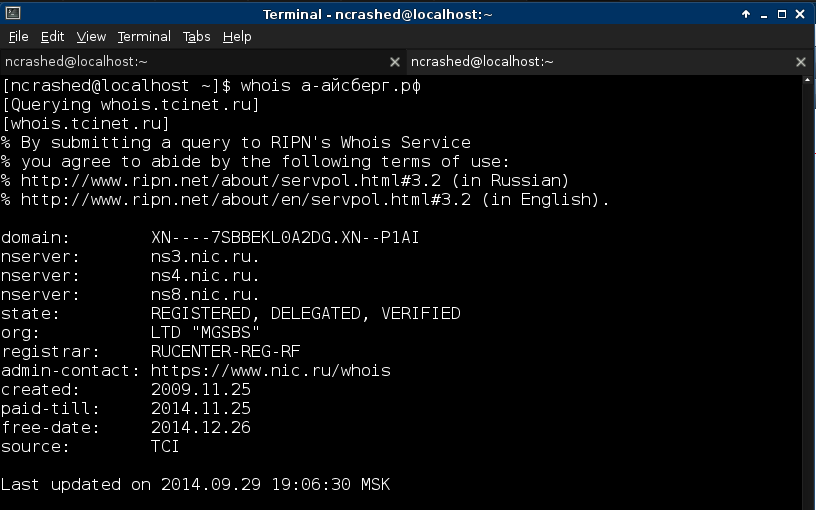
\includegraphics[width=0.7\textwidth]{009}
\end{figure}
Вся информация получена из базы данных Internet Network Information Center - interNIC.

Сделаем запрос lookup:
\begin{figure}[h!]
\centering
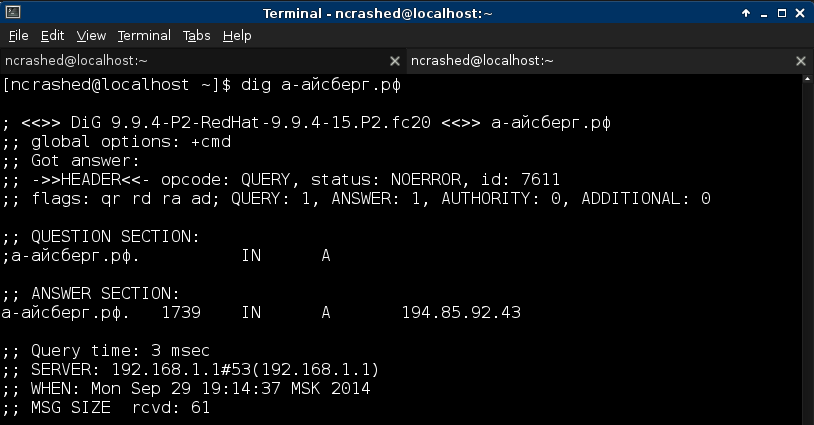
\includegraphics[width=0.7\textwidth]{010}
\end{figure}
DNS сервер ответил, что домен а-айсберг.рф имеет IP адрес 194.85.92.43.

Произведем HTTP запрос на а-айсберг.рф:
\begin{figure}[h!]
\centering
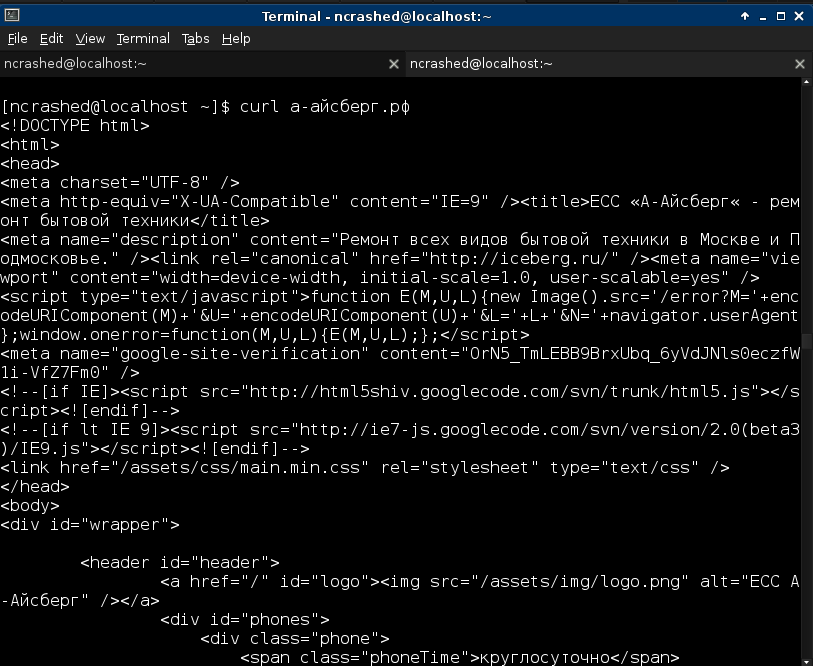
\includegraphics[width=0.7\textwidth]{011}
\end{figure}
\clearpage

Проанализируем запрос в пакетном анализаторе:
\begin{figure}[h!]
\centering
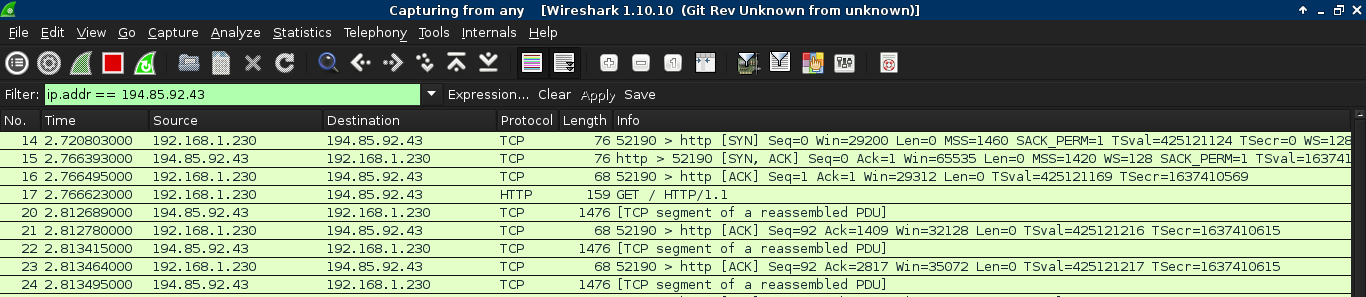
\includegraphics[width=\textwidth]{012}
\end{figure}

Соединение производится по трехэтапной процедуре (SYN-SYN-ACK-ACK), называемой three-way handshake. Далее идет передача данных страницы с подтверждением на каждую часть.

\begin{figure}[h!]
\centering
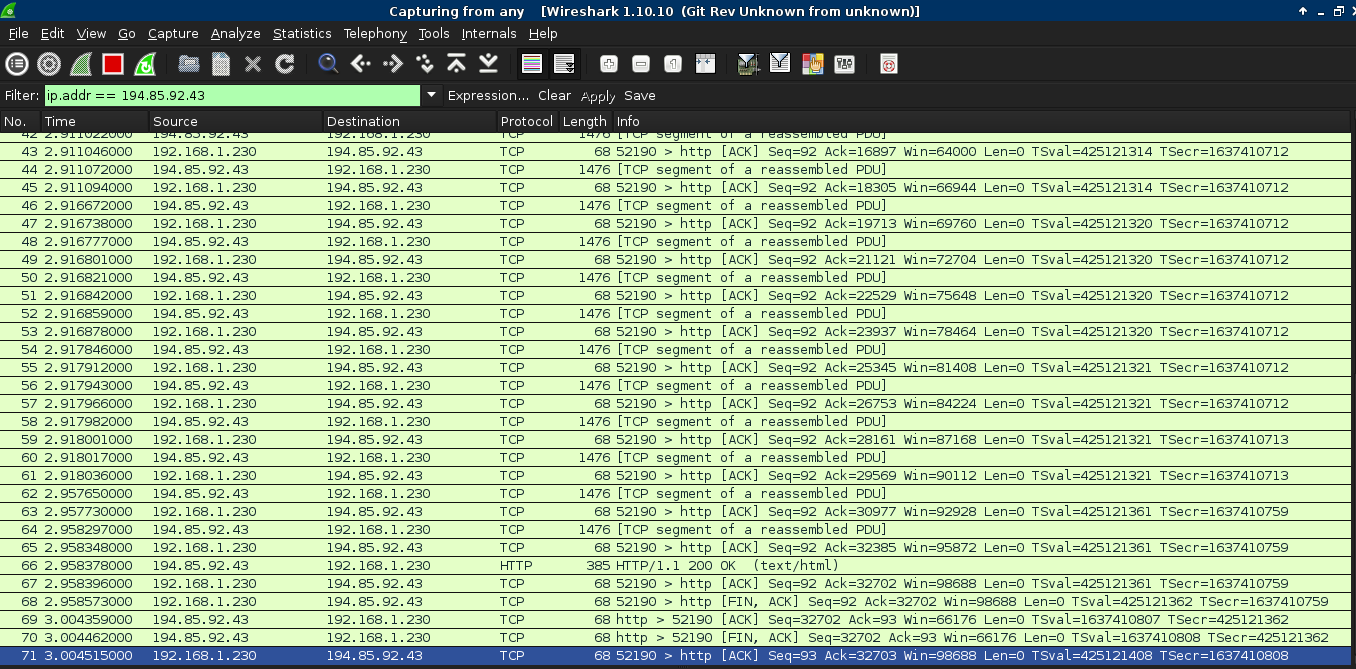
\includegraphics[width=\textwidth]{013}
\end{figure}

Завершение соединения производится в четыре этапа (по два на каждое направление передачи, так как виртуальный канал полнодуплексный). Последовательность сообщений: FIN, ACK-ACK-FIN, ACK-ACK.

%\begin{longtable}{p{1cm}|p{2cm}|p{2cm}|p{2cm}|p{2cm}|p{2cm}|p{1.5cm}|p{1.5cm}}
%\caption{Исходные данные для выполнения курсовой работы.}
%\label{tab:task} \\
%№  & Цент-ральный офис & 1-ый филиал & 2-ой филиал & СУБД и выбор оборудования & Диски сервера & Диски сервера & Модель \\ 
%\hline 
%8 & 5(1)/2(1) & 3(3)/2(3) & \centering 18 & 23/33/43 & \centering 53 & 64 (5) (0.9) & \centering 73 \\ 
%\end{longtable}


\end{document}